%!TEX program = xelatex
\documentclass[letterpaper,12pt]{exam}
\usepackage{../videoNotes}
\usepackage{xcolor}
\usepackage[dvipsnames]{xcolor}
\usepackage{soul}
\usepackage{tabulary}
\usepackage{fontspec}

%\usepackage{draftwatermark}
%\SetWatermarkText{Draft}
%\SetWatermarkScale{1.5}
%\SetWatermarkColor{red!20}

\newcommand{\unit}{Unit 08}
\pagestyle{headandfoot}
\firstpageheader{CSC 264 \semester\ \  \unit}{}{Name: $\rule{6cm}{0.15mm}$}
\runningheader{CSC 264 \semester}{\unit}{Page \thepage\ of \numpages}
\firstpagefooter{}{}{}
\runningfooter{}{}{}

\begin{document}

%\underconstruction

\par{\fontfamily{qzc}\selectfont\textbf{}}
\begin{questions}

\section*{\unit\_010 -- Declaring multiples }
\begin{samepage}
    \question What is an address?
    \vspace{5mm}
\end{samepage}
\par
\begin{samepage}
    \question In the listing we see text like the following.  If we execute the program, will char3 be loaded at location 0003 in physical memory?  Explain.
\begin{verbatim}
    0003 43                char3: .byte 67  # same as 0x43
\end{verbatim}
    \vspace{5mm}
\end{samepage}
\par
\begin{samepage}
    \question We have been using the term "variable" this semester.  How are they similar to the idea of a variable in a high level language?  How are they different? (I did not cover this explicitly in the video.  Think about it.)
    \vspace{5mm}
\end{samepage}
\begin{samepage}
    \question What does \$ mean when it appears before a label?
    \vspace{5mm}
\end{samepage}
\par
\begin{samepage}
    \question What does it mean when a register appears in (parenthesis)?
    \vspace{5mm}
\end{samepage}
\par
 \begin{samepage}
     \question How are the \$ and () compliments of each other?
     \vspace{5mm}
 \end{samepage}
 \par
\begin{samepage}
    \question Explain the difference between the following two lines of code.  What would be loaded into the register in each?  Also, why doesn't (\%rdx) change?
    \begin{verbatim}
   movb (%rbx), %dil
   movq (%rbx), %rdi

    \end{verbatim}
    \vspace{5mm}
\end{samepage}
\par
   \section*{\unit\_020 -- Arrays}
   \par{\fontfamily{qzc}\selectfont\textbf{Video Length 8:10}}
   \begin{samepage}
       \question Use commas to declare an array of 3 integers as quads.  
       \vspace{5mm}  
   \end{samepage}
   \par
   \begin{samepage}
       \question Given the array in the question above, write the code needed to create a variable that will calculate the size of the array.
       \vspace{5mm}
   \end{samepage}
   \par
\begin{samepage}
    \question Given the array and the array size calculated above, how many bytes will be stored as the size?
    \vspace{5mm}
\end{samepage}
\par
\begin{samepage}
    \question For review, fill in the right column of the following table.  
   \begin{center}
\begin{tabular}{ |c| c| }
 size & declaration  \\
 \hline 
 {\large 1} & \textcolor{blue}{\casual .byte} \\  
 {\large 2} &  \\    
 {\large 4} &  \\
 {\large 8} &  \\
\end{tabular}
\end{center}
    \vspace{5mm}

\end{samepage}
\par
 
 
   \rule{0.5\textwidth}{.4pt} %End of section
   %----------------------------------
 \section*{\unit\_ 030 -- Addressing Modes}

\begin{samepage}
    \question Memory modes are about the \rule{1cm}{0.15mm}\rule{1cm}{0.15mm} of an instruction
    \vspace{5mm}
\end{samepage}
\par
  \begin{samepage}
     \question What are the three basic addressing modes?
     \vspace{5mm}
 \end{samepage}
 \par


\begin{samepage}
    \question What is immediate mode?  How can you recognize immediate mode in GAS assembler?
    \vspace{5mm}
\end{samepage}
\par
 \begin{samepage}
     \question How do you recognize that an operand is Register mode in GAS assembler?
     \vspace{5mm}
 \end{samepage}
 \par
\begin{samepage}
    \question Which of the three modes involves calculation of an address?
    \vspace{5mm}
\end{samepage}
\par
\begin{samepage}
    \question For each of the following, write I for immediate mode, R for register mode, or M for Memory mode.  Assume "number" is a label.
\begin{itemize}
    \item \$99
    \item \%rdx
    \item (\%rax)
    \item \$number
    \item number
\end{itemize}
    \vspace{5mm}
\end{samepage}
    \rule{0.5\textwidth}{.4pt} %End of section
 %----------------------------------
\section*{\unit\_040 -- Memory Addressing Modes}
\begin{samepage}
    \question Fill in the blanks in the following:
    \par
    $address = \rule{2.5cm}{0.15mm}(\rule{2.5cm}{0.15mm},\rule{2.5cm}{0.15mm},\rule{2.5cm}{0.15mm})$
    \vspace{5mm}
\end{samepage}
\par
\begin{samepage}
    \question Is the value added to or multiplied by the fields in parenthesis
    \vspace{5mm}
\end{samepage}
\par
 
\begin{samepage}
    \question In the formula above, which two fields must be registers?
    \vspace{5mm}
\end{samepage}
\begin{samepage}
    \question What values are allowed for the multiplier?
    \vspace{5mm}
\end{samepage}
\par
\begin{samepage}
    \question What is the default number if the value field is omitted? 
    \vspace{5mm}
\end{samepage}
\par
\begin{samepage}
    \question What is the default number if the basereg field is omitted? 
    \vspace{5mm}
\end{samepage}
\begin{samepage}
    \question What is the default number if the idxreg field is omitted? 
    \vspace{5mm}
\end{samepage}
\begin{samepage}
    \question What is the default number if the multiplier is omitted? 
    \vspace{5mm}
\end{samepage}

      
\rule{0.5\textwidth}{.4pt} %End of section
%----------------------------------
\section*{\unit\_050 -- Printing a byte the hard way}
\begin{samepage}
    \question What would need to be changed in the following block of code to get it to prink the "n" in skunk?
\begin{verbatim}
    .data
    format:.asciz "The char is \'%c\'.\n"
    animal:.ascii "skunk","\0"
.text
main:
   movq \$animal, \%r15
   movq \$0, \%r14
   xor \%rax, \%rax
   movq \$format, \%rdi
   movb (\%r15,\%r14), \%sil
   call printf
\end{verbatim}

\end{samepage}
\par
\rule{0.5\textwidth}{.4pt} %End of section
%----------------------------------
\section*{\unit\_055 -- Printing bytes with a loop }
\par{\fontfamily{qzc}\selectfont\textbf{Video Length }}
\begin{samepage}
    \question Modify the text part of the code from the previous question so that it will print all of the characters in animal.  Just do the main: label up until the \_exit label.
    \vspace{65mm}
\end{samepage}

\rule{0.5\textwidth}{.4pt} %End of section
%----------------------------------
\section*{\unit\_060 -- Looping Quads }
\begin{samepage}
    \question Suppose you want to skip the \[0\] year. Modify the following line of code so that it would skip the first year.
    \begin{verbatim}
          movq (\%r15,\%r14,8), %rdx
    \end{verbatim}
    \vspace{5mm}
\end{samepage}
\par
\rule{0.5\textwidth}{.4pt} %End of section
%----------------------------------

\section*{\unit\_070 -- RIP Relative Addressing}
\begin{samepage}
    \question What are two things that RIP Relative addressing accomplishes?
    \vspace{5mm}
\end{samepage}
\par

\begin{samepage}
    \question What is the difference between PIC and PIE?
    \vspace{5mm}
\end{samepage}
\par
\begin{samepage}
    \question In the following code, change the line or lines that need to be modified for PIC.  
    \begin{verbatim}
    .data
        ages: .quad 10, 23, 8, 9, 23
        agesN .quad 5
    .text
    main:
       movq ages, %r8
       movq agesN, %r9
       xorg %rax, %rax
       movq $ages %rdi     
    \end{verbatim}
\end{samepage}
\par
 
\rule{0.5\textwidth}{.4pt} %End of section
%----------------------------------




%----------------------------------
\end{questions} 
%footer
\begin{center}
    \rule{0.667\textwidth}{.8pt} %End of section
\end{center}


If you have any lingering questions or problems, please write them here or see me.
\vfill
\begin{center}
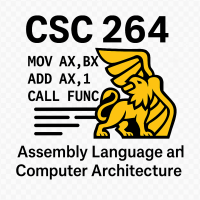
\includegraphics{../csc264Logo}
\end{center}
\end{document} 